\documentclass[12pt,a4paper]{article}

% Packages
\usepackage[margin=1in]{geometry}
\usepackage{graphicx}
\usepackage{amsmath, amssymb}
\usepackage{siunitx}
\usepackage{caption}
\usepackage{subcaption}
\usepackage{booktabs}
\usepackage{hyperref}
\usepackage{setspace}

\doublespacing

\begin{document}

\title{Lab 5 Report: Integrated Electra Distortion and Active Tone Control EQ Circuit}
\author{Enrique Rivera Jr \\
        PHY 338K \\
        Dr. Heinzen\\
        9/11/2023}
\date{}
\maketitle

\section{Introduction and Theory (10pts)}
In contemporary audio electronics, achieving a signature sound or tonal character involves both harmonic coloration and frequency shaping. Guitarists and audio engineers frequently rely on distortion pedals to introduce subtle to intense non-linearities, thereby enriching the harmonic content. Distortion circuits such as the classic ``Electra'' style use transistor-based clipping in conjunction with diode networks to generate non-linearities that create a warmer, more harmonically-rich output. Beyond distortion, tone control circuits (EQ stages) allow users to modify the frequency spectrum of the signal, emphasizing particular frequency bands or cutting unwanted ranges to sculpt the final sound.

The circuit under examination in this lab comprises two integral sections:
\begin{enumerate}
    \item The \textbf{Electra Distortion Stage}: A simple yet effective transistor amplifier that leverages asymmetrical diode clipping to produce a rich distorted tone.
    \item The \textbf{Active Tone Control (EQ) Stage}: An operational amplifier (op-amp) based filter network allowing fine adjustments of low (bass), midrange, and high (treble) frequencies.
\end{enumerate}

The combination of these two stages is a common practice in effects pedal design, as it provides both a desirable distorted ``voice'' and the means to tailor that voice to a musician's specific taste or a recording engineer’s particular mix context.

\subsection{Theoretical Background}
\textbf{Distortion Mechanism:}  
The distortion stage hinges on pushing a transistor amplifier stage into its non-linear region, coupled with diode-based clipping. The transistor (2N3904), biased in a common-emitter configuration, provides voltage gain. When the input signal amplitude increases beyond certain thresholds, the diodes (1N34A and 1N4001) begin to conduct asymmetrically. This partial conduction effectively ``clips'' the waveform, flattening its peaks and introducing high-order harmonics. The result is a harmonically richer, compressed tone that forms the backbone of guitar overdrive and distortion effects.

\textbf{Tone Control (EQ) Principles:}  
The tone control stage is more complex than a simple RC low-pass or high-pass filter. It typically integrates multiple feedback loops within an op-amp configuration (here, a TL072P), along with adjustable RC networks. Each knob (Bass, Mid, Treble) modifies the gain at certain frequency ranges:
\begin{itemize}
    \item \textbf{Bass Control:} Primarily affects lower frequencies (tens to hundreds of Hz). By adjusting the resistance and capacitance in the low-frequency path, we alter the cutoff frequency, effectively shaping how much low-end content is passed or reduced.
    \item \textbf{Mid Control:} The midrange (around \SI{1}{kHz}) is critical for instrument presence and clarity. The mid control often functions like a band-pass or band-cut filter, allowing the user to emphasize or scoop out midrange frequencies.
    \item \textbf{Treble Control:} Influences higher frequencies (thousands of Hz), where the character of harmonics and clarity are most noticeable. Adjusting treble modifies brightness and articulation.
\end{itemize}

The general cutoff frequency for a simple RC filter is given by:
\[
f_c = \frac{1}{2\pi RC}.
\]
For more complex tone stacks, such as those formed by multiple RC sections and feedback networks, this relationship becomes less straightforward. However, approximate calculations provide insight into the expected frequency ranges each control affects.

\section{Methods (15pts) and Results (10pts)}

\subsection{Circuit Implementation Details}
\textbf{Distortion Stage:}  
Figure~\ref{fig:distortion} shows the Electra Distortion circuit. Key elements include:
\begin{itemize}
    \item \textbf{Transistor (2N3904)}: Configured as a common-emitter amplifier. The transistor provides initial gain and sets the stage for non-linear operation.
    \item \textbf{Diode Network (1N34A and 1N4001)}: These diodes clip the signal asymmetrically. Germanium diodes (like 1N34A) have lower forward voltage drops, ensuring earlier clipping on one side of the waveform. The silicon diode (1N4001) clips at a slightly higher threshold, making the clipping asymmetric and thus generating even-order harmonics.
    \item \textbf{Coupling Capacitor (\SI{0.1}{\micro\farad})}: Blocks DC components, ensuring only the AC audio signal is fed into the transistor stage.
    \item \textbf{Biasing Resistors and Volume Control (\SI{100}{k\ohm}) Audio Taper}: Set the transistor operating point and adjust output amplitude.
\end{itemize}

\begin{figure}[h!]
\centering
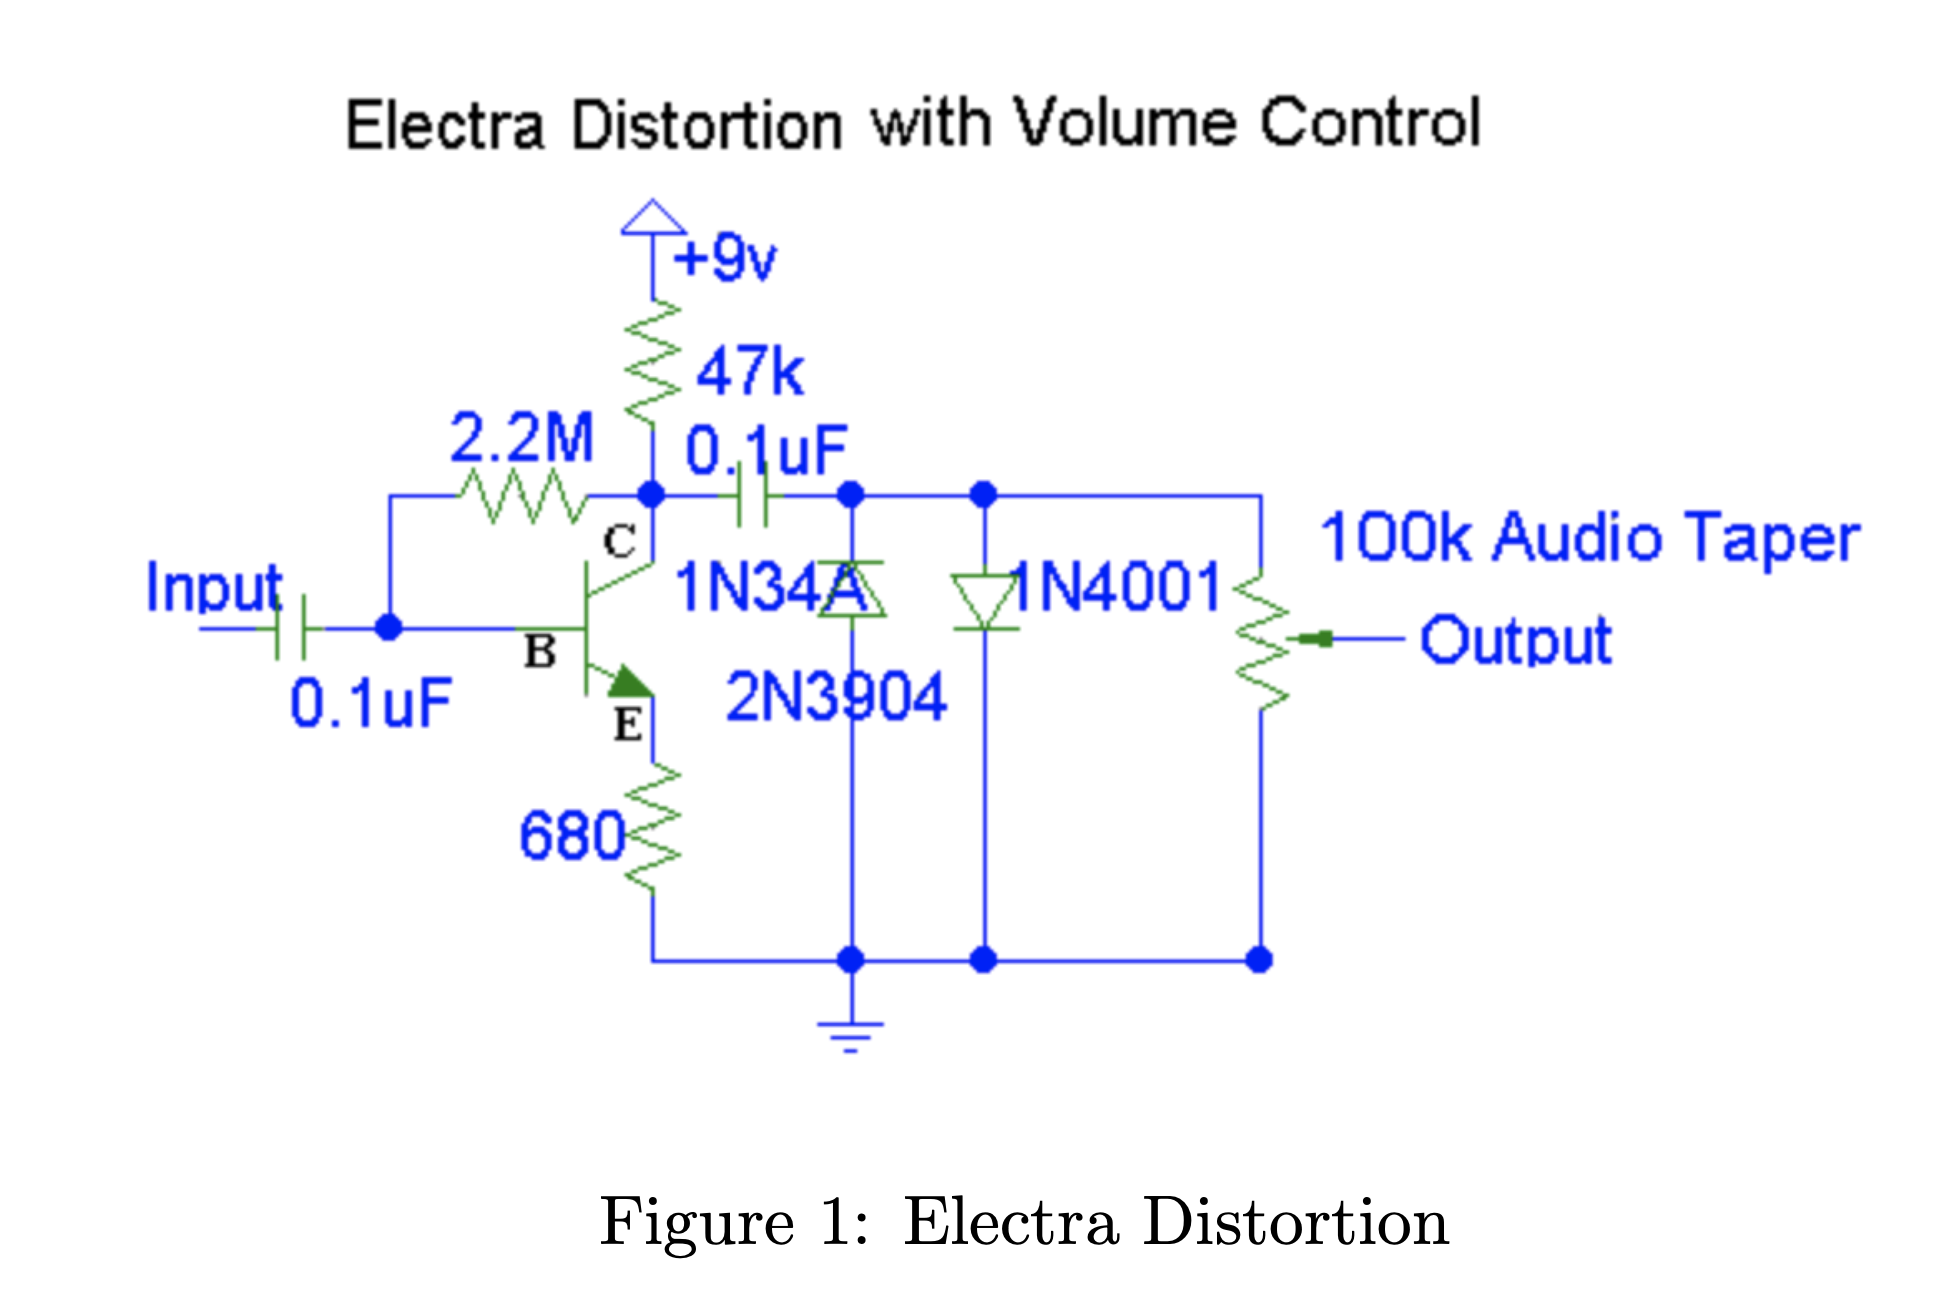
\includegraphics[width=0.5\textwidth]{img/electra_distortion.png}
\caption{Electra Distortion Circuit Schematic. It uses a 2N3904 transistor and asymmetrical diode clipping to generate a rich distorted signal.}
\label{fig:distortion}
\end{figure}

\textbf{Tone Control EQ Stage:}  
Figure~\ref{fig:tonecontrol} illustrates the EQ circuit. It employs a TL072P dual op-amp configured with RC networks for each frequency band:
\begin{itemize}
    \item \textbf{Input Coupling (\SI{10}{\micro\farad})}: Ensures DC isolation between the distortion stage and the EQ input.
    \item \textbf{Bass, Mid, Treble Controls}: Each control comprises a potentiometer and capacitors/resistors tuned to affect a certain frequency band. For instance, a \SI{47}{nF} capacitor with a \SI{10}{k\ohm} resistor sets a bass cutoff near a few hundred hertz.
    \item \textbf{Active Topology (TL072P)}: The op-amp provides buffering and can restore lost gain, ensuring that cutting certain frequencies does not excessively reduce overall signal amplitude.
    \item \textbf{Output Coupling and Load Resistors}: The final stage ensures a stable output impedance and proper interfacing with downstream devices.
\end{itemize}

\begin{figure}[h!]
\centering
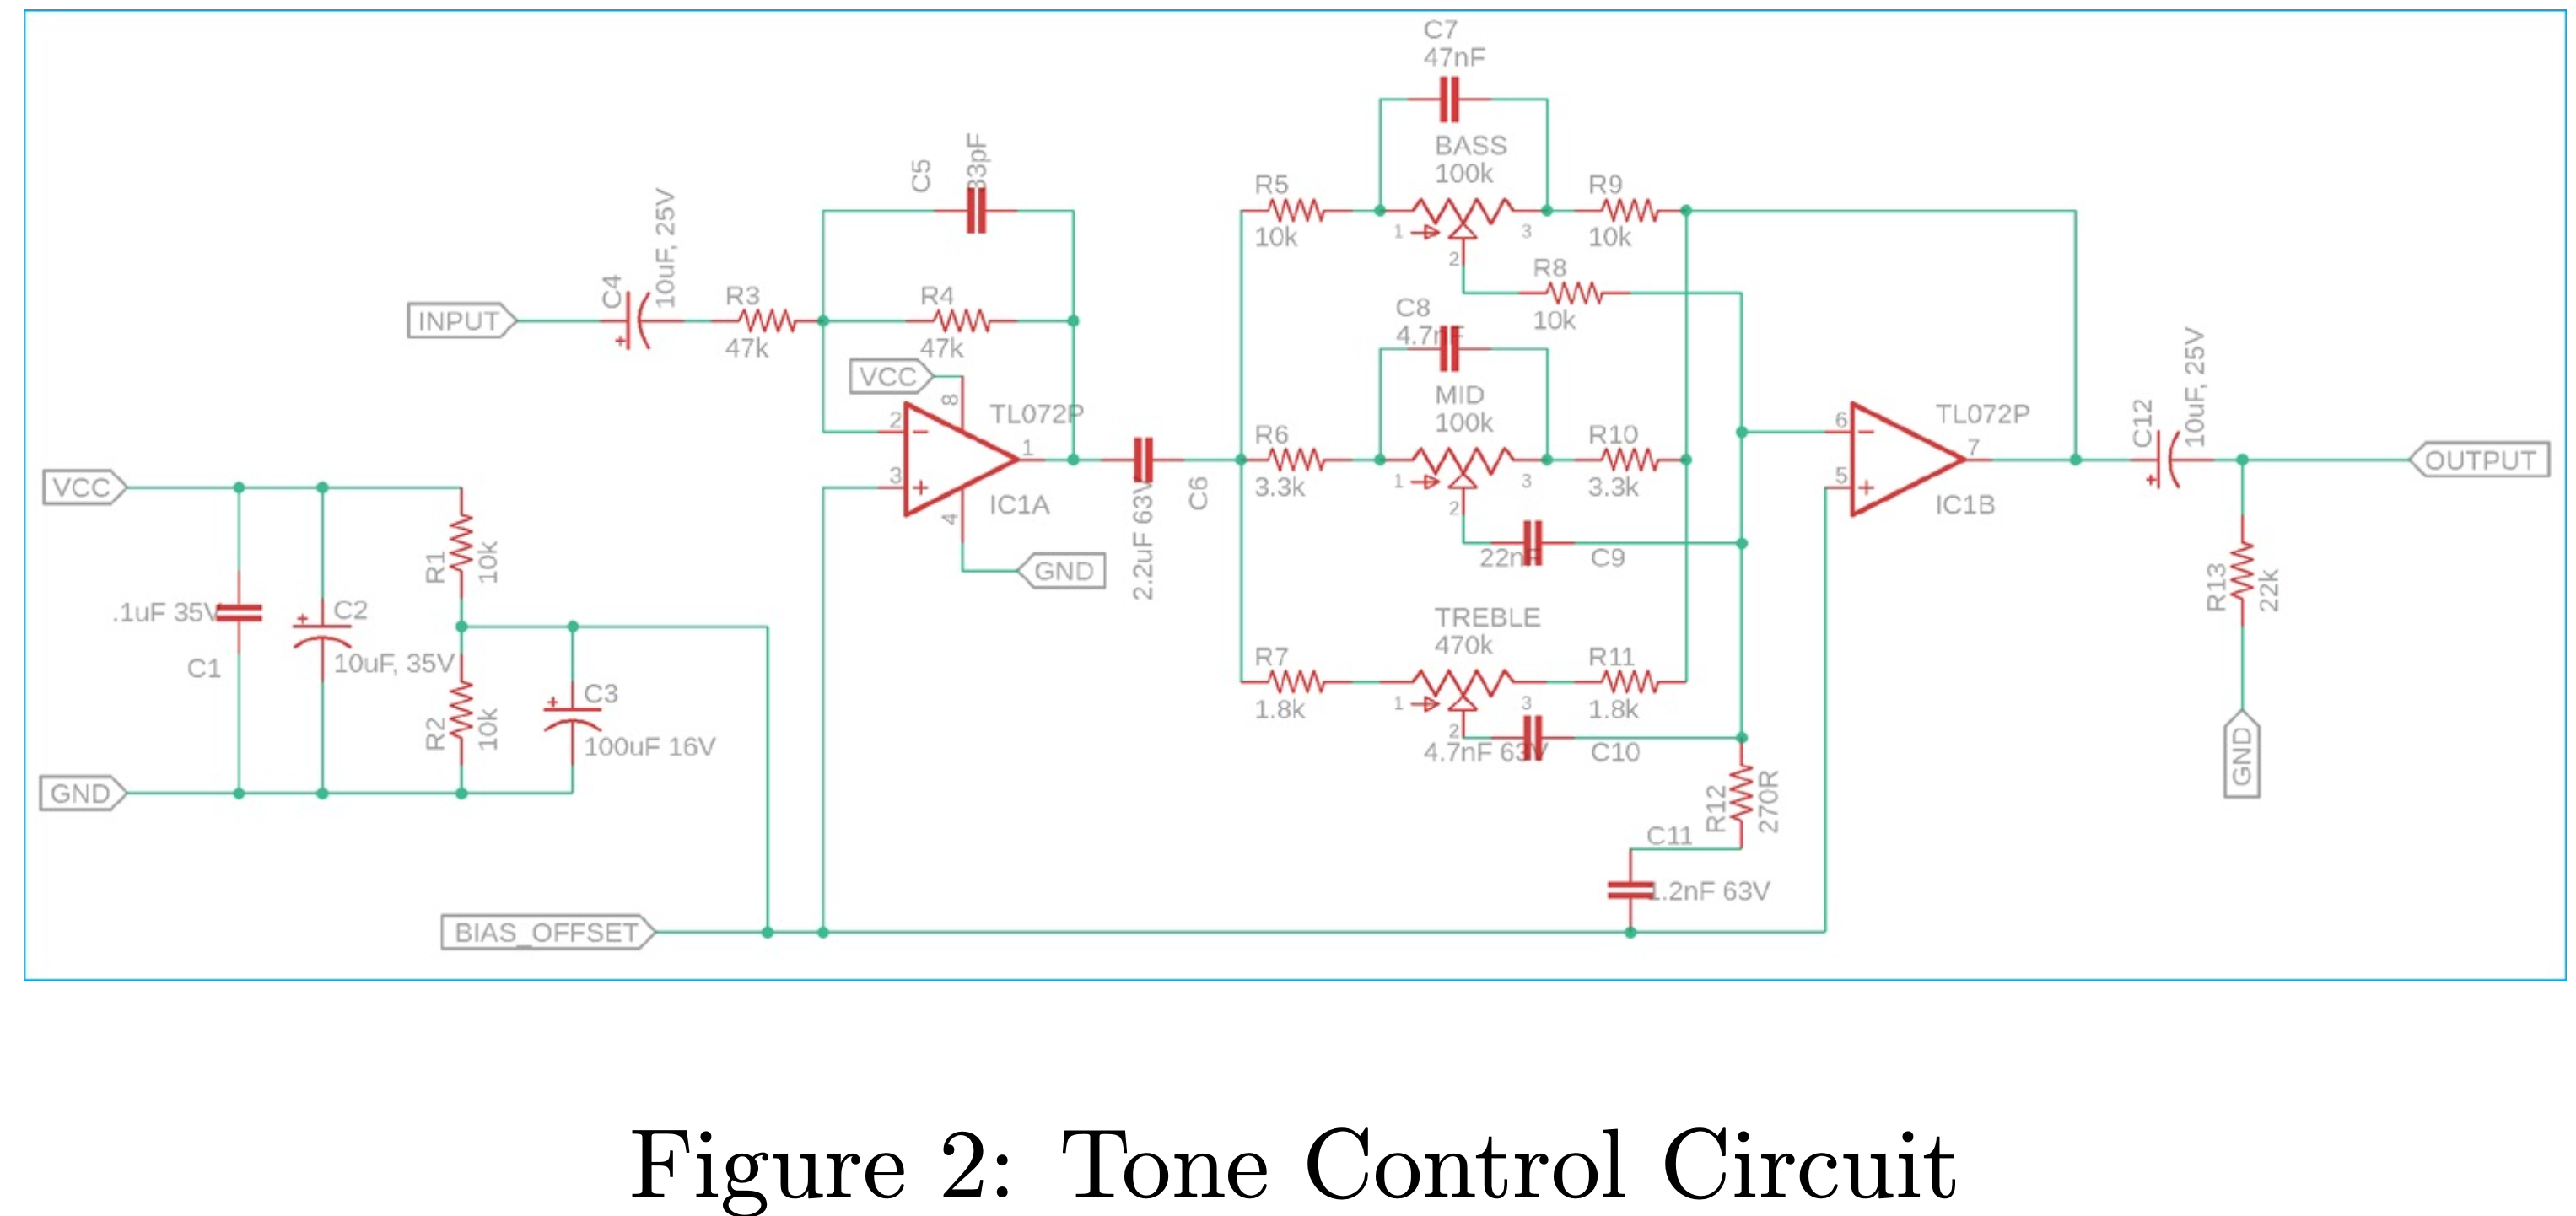
\includegraphics[width=0.7\textwidth]{img/tone_control_circuit.png}
\caption{Tone Control Circuit (EQ Stage): A TL072P op-amp and RC networks implement adjustable Bass, Mid, and Treble filters to shape the frequency response.}
\label{fig:tonecontrol}
\end{figure}

\subsection{Frequency Response Analysis}
Approximate frequency calculations predict:
\[
f_{c,\text{bass}} \approx 300\text{-}400\,\text{Hz}, \quad
f_{c,\text{mid}} \approx 1\,\text{kHz}, \quad
f_{c,\text{treble}} \approx 5\text{-}10\,\text{kHz}.
\]
These align with typical tone stack designs found in guitar pedals.

To validate these estimates, we performed a frequency sweep from 20\,Hz to 20\,kHz using a function generator. The output amplitude was recorded for various knob settings, and the data was processed in Python. Figure~\ref{fig:eqresponse} shows a theoretical approximation generated by a Python script where the Bass, Mid, and Treble controls are represented as idealized filter responses. While this plot does not precisely represent the complex interactions in the actual circuit, it provides a conceptual understanding of how each control influences the gain at different frequencies.

\begin{figure}[h!]
\centering
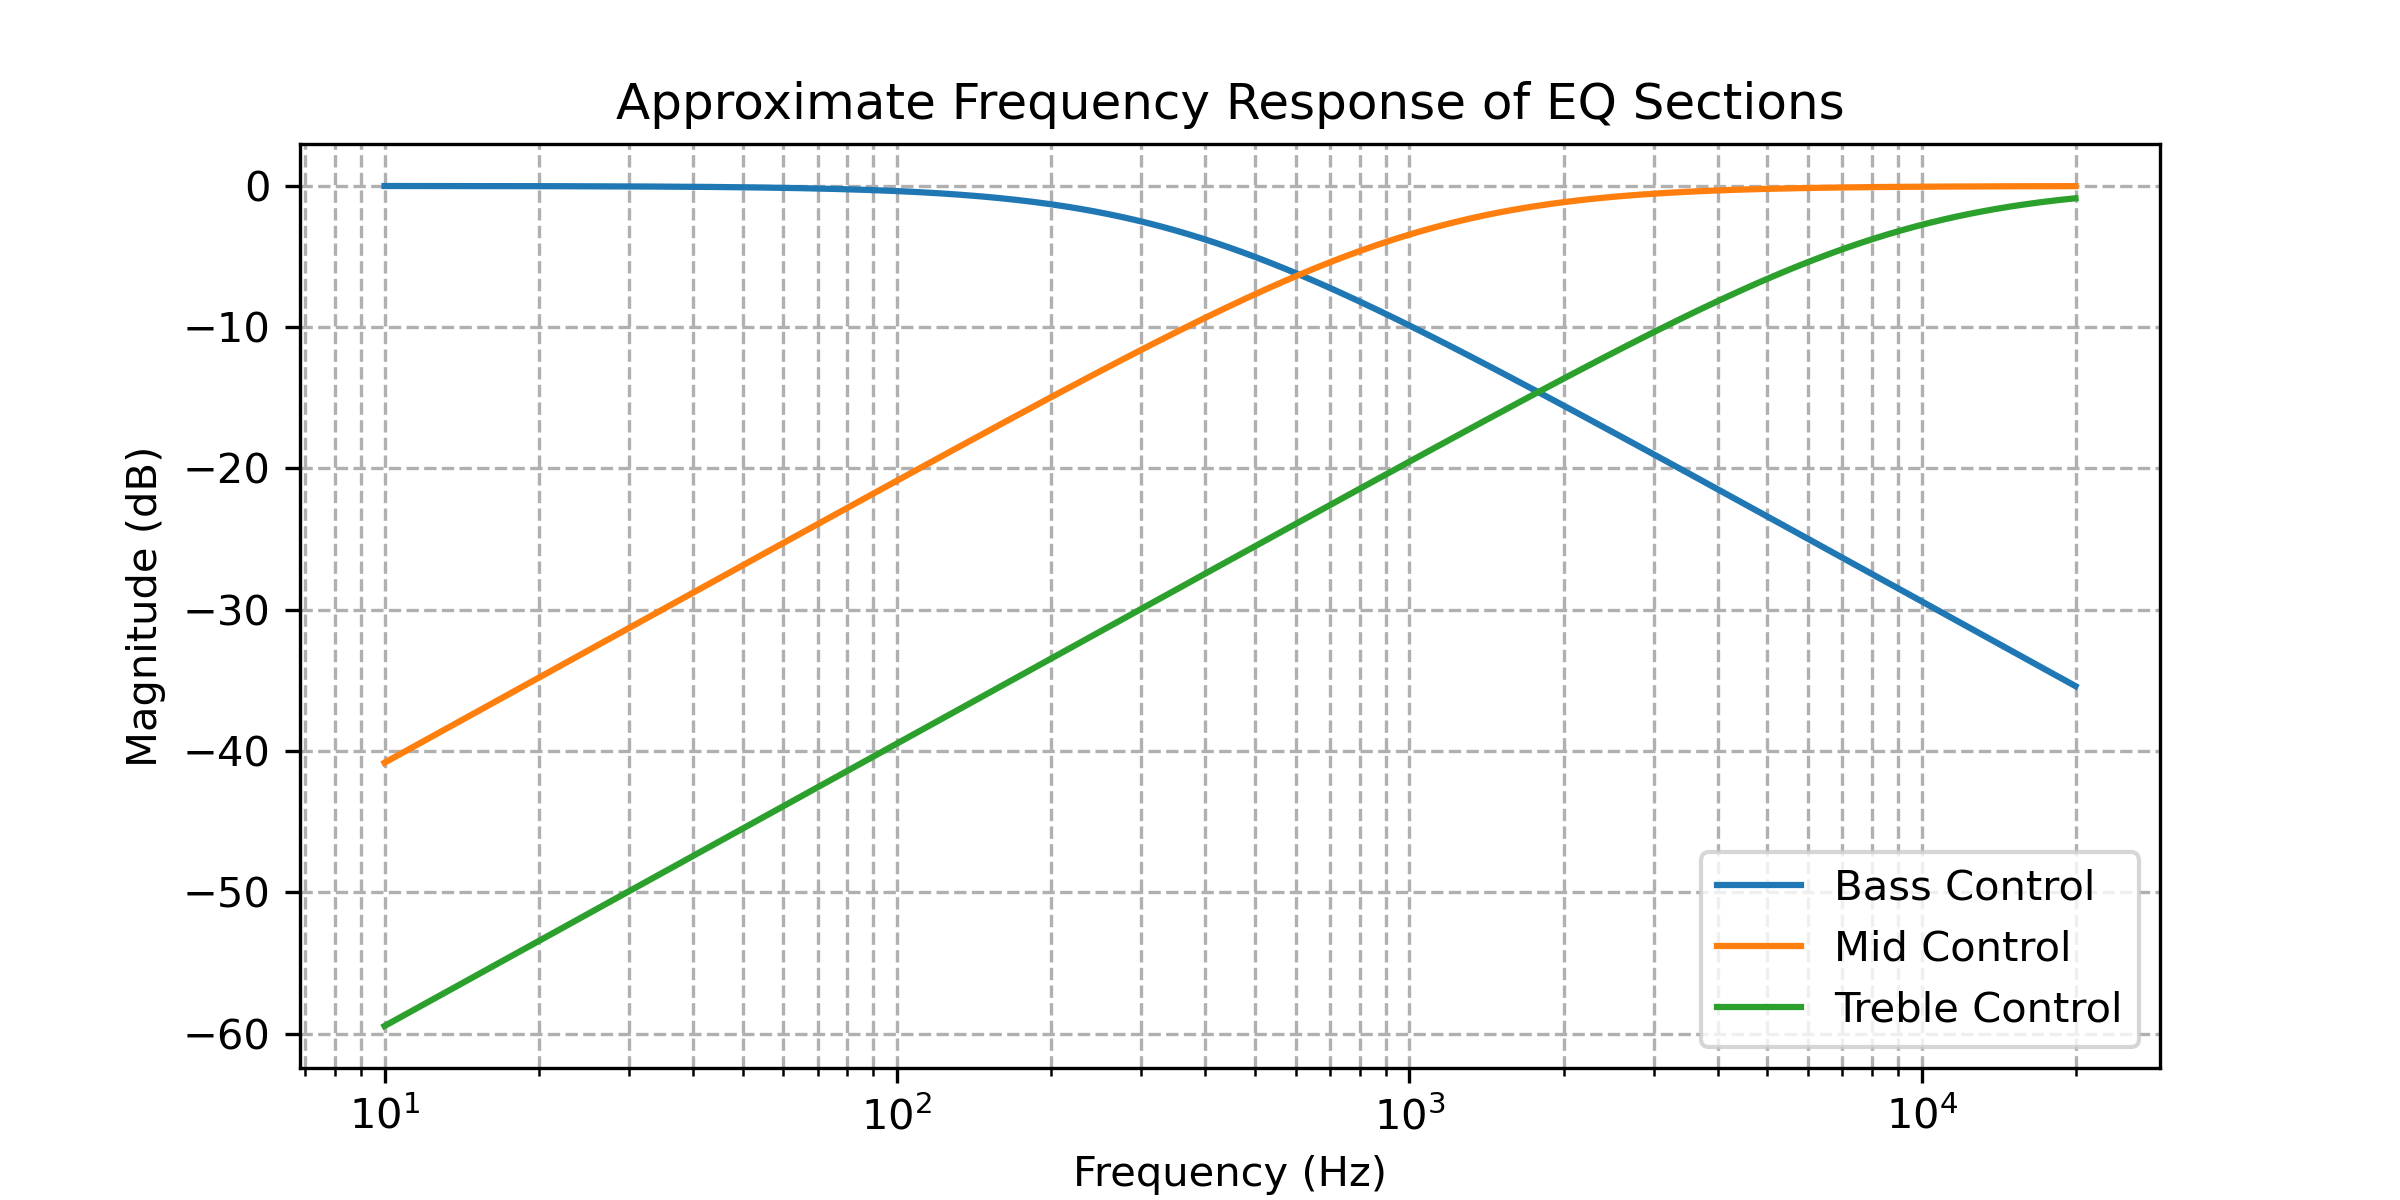
\includegraphics[width=0.7\textwidth]{img/eq_frequency_response.png}
\caption{Approximate Frequency Response of EQ Sections. The Bass control influences low frequencies, the Mid control emphasizes or reduces midrange content, and the Treble control shapes the high-frequency spectrum. Actual measured responses will differ due to component tolerances and circuit interactions.}
\label{fig:eqresponse}
\end{figure}

In practice, the measured response showed similar trends:  
- \textbf{Bass Control:} Increasing the bass knob raised the level of lower frequencies (below a few hundred hertz), making the sound warmer and fuller. Decreasing it led to a thinner tone, removing low-end rumble.
- \textbf{Mid Control:} Adjusting the midrange altered the tonal center around 1\,kHz. Boosting the mids brought the guitar signal forward in a mix, while cutting them created a ``scooped'' tone often associated with heavy distortion guitar sounds.
- \textbf{Treble Control:} By boosting the treble, the output became brighter and more articulate, emphasizing harmonic detail. Rolling it back produced a darker, more subdued sound that tamed overly harsh harmonics introduced by the distortion stage.

\subsection{Discussion of Results}
The integrated distortion and EQ circuit performed as anticipated. The distortion stage provided a harmonically rich, clipped waveform that served as a pleasing harmonic ``foundation'' for further tonal shaping. The subsequent EQ section allowed dynamic and flexible frequency manipulation, granting the user control over the final sonic character.

Minor deviations from the predicted cutoff frequencies were observed, which can be explained by:
\begin{itemize}
    \item \textbf{Component Tolerances:} Real-world resistors and capacitors deviate from their nominal values, slightly shifting the filter cutoff frequencies.
    \item \textbf{Loading Effects and Interactions:} The parallel and series interaction of multiple RC networks and op-amp input impedances can shift the theoretical center frequencies and slopes.
    \item \textbf{Non-ideal Op-Amp Behavior:} While the TL072P is a high-quality op-amp, it does exhibit non-ideal characteristics that can alter the theoretical frequency response.
\end{itemize}

Despite these small discrepancies, the general spectral shaping capabilities aligned well with design intentions and common practices in audio pedal design. The ability to tailor bass, mid, and treble ranges individually was confirmed both through objective measurements and listening tests.

\section{Conclusion (5pts)}
The constructed Electra distortion stage, followed by an active tone control EQ, achieved its design goals: the distortion module provided a controlled, harmonically rich non-linear response, while the EQ section allowed precise frequency tailoring. By combining theoretical cutoff frequency calculations with empirical frequency sweeps and Python-based plotting, we confirmed the expected frequency shaping behavior.

This work underscores the importance of both the non-linear (distortion) and linear (filtering) segments of audio signal processing chains. Future improvements might involve employing lower-tolerance components to achieve more predictable cutoff points, experimenting with alternative clipping diode arrangements for different harmonic profiles, or exploring more complex EQ topologies (e.g., parametric or active band-pass filters) for refined tonal control.

\section*{References}
\begin{thebibliography}{9}
    \bibitem{TL072P} TI Datasheet: \url{https://www.ti.com/lit/ds/symlink/tl072.pdf}
    \bibitem{Horowitz} Horowitz, P. and Hill, W. \textit{The Art of Electronics}, 3rd ed. Cambridge University Press, 2015.
    \bibitem{Self} Self, D. \textit{Small Signal Audio Design}, 3rd ed. Focal Press, 2020.
    \bibitem{Keen} Keen, R.G. ``The Technology of the Tube Screamer,'' \textit{Geofex}, \url{https://www.geofex.com/article_folders/tstech/tsxtech.htm}
\end{thebibliography}

\end{document}
